\begin{center}
	
	
	\tikzset{every picture/.style={line width=0.75pt}} %set default line width to 0.75pt        
	
	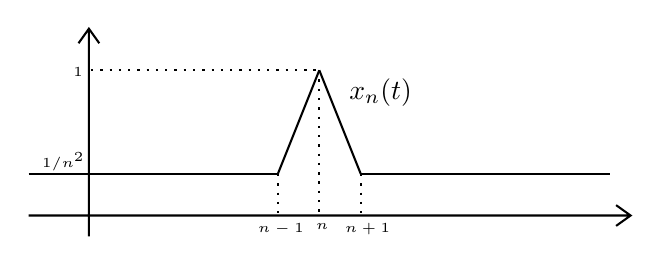
\begin{tikzpicture}[x=0.75pt,y=0.75pt,yscale=-1,xscale=1]
		%uncomment if require: \path (0,300); %set diagram left start at 0, and has height of 300
		
		%Shape: Axis 2D [id:dp1663102831517027] 
		\draw  (100,160) -- (390,160)(129,70) -- (129,170) (383,155) -- (390,160) -- (383,165) (124,77) -- (129,70) -- (134,77)  ;
		%Straight Lines [id:da8094250901048163] 
		\draw    (100,140) -- (220,140) ;
		%Straight Lines [id:da3926524751184308] 
		\draw    (220,140) -- (240,90) ;
		%Straight Lines [id:da9345956516168132] 
		\draw    (260,140) -- (240,90) ;
		%Straight Lines [id:da2510520175171027] 
		\draw    (260,140) -- (380,140) ;
		%Straight Lines [id:da6251110538749508] 
		\draw  [dash pattern={on 0.84pt off 2.51pt}]  (240,90) -- (240,160) ;
		%Straight Lines [id:da5544158951216948] 
		\draw  [dash pattern={on 0.84pt off 2.51pt}]  (220,140) -- (220,160) ;
		%Straight Lines [id:da20393290290096278] 
		\draw  [dash pattern={on 0.84pt off 2.51pt}]  (260,140) -- (260,160) ;
		%Straight Lines [id:da6458699328315521] 
		\draw  [dash pattern={on 0.84pt off 2.51pt}]  (130,90) -- (240,90) ;
		
		% Text Node
		\draw (120,87.4) node [anchor=north west][inner sep=0.75pt]  [font=\tiny]  {$1$};
		% Text Node
		\draw (209,162.4) node [anchor=north west][inner sep=0.75pt]  [font=\tiny]  {$n-1$};
		% Text Node
		\draw (251,162.4) node [anchor=north west][inner sep=0.75pt]  [font=\tiny]  {$n+1$};
		% Text Node
		\draw (237,162.4) node [anchor=north west][inner sep=0.75pt]  [font=\tiny]  {$n$};
		% Text Node
		\draw (253,92.4) node [anchor=north west][inner sep=0.75pt]    {$x_{n}( t)$};
		% Text Node
		\draw (105,128.4) node [anchor=north west][inner sep=0.75pt]  [font=\tiny]  {$1/n^{2}$};
		
		
	\end{tikzpicture}
\end{center}